
% Package for chemical equation typesetting
\chapter{Introduction}
In this chapter an introduction to the geothermal wells along with an introduction to scaling and its effects is given followed by some relevant chemical reactions and their properties. 

\section{Introduction to Geothermal Wells}
\newline \newline
As of 2040, Energy Information Administration (EIA) expects an increase of 28\% in world energy consumption. The majority of this consumption is projected to account from developing countries such as India, China and other third world countries since the economy is increasing rapidly. \cite{EIA}

In order to overcome this fast increase, the human kind cannot rely only on fossil fuels and other sustainable technologies like solar, wind, geothermal are required. However, the emmision of CO$_2$ is also increasing from 6000 million metric tons carbon in year 2000 to 10000 million metrics tons in 2010. That's why many countries such as Denmark, Norway, Germany, The Netherlands etc., are moving away from traditional fuel sources to the new energy. One of these energy is Geothermal energy. 
\newline\newline
As the name suggests, \textit{Geothermal} comes from the greek work, \textit{geo}: which means Earth and \textit{therma} meaning heat. 
Geothermal energy is the fraction of the natural heat of the Earth that is transported by the magma flow, conduction or/and convection from the Earth surface to the drilling range of the surface. The heat comes from the decay of the natural radioactive material that is transmitted to the surface from the molten core in the earth. It has been estimated that about 42 million megawatts of power flow from earth’s interior by conduction.\cite{Stef}
\newline\newline

It is important to mention that there are mainly two types of geothermal resources: Low Temperature and High Temperature Resources. Low temperature resources are less than 180 degree C and are enough to supply only heating whereas high temperature resources (more than 180 degree C) are hot enough to generate electricity. The High Temperature resources supply about 99\% of its geothermal energy and are considered in this report. \cite{Sae2013}

\section{Introduction to Scaling}
\newline \newline

Despite the fact that geothermal is one clean energy and almost CO$_2$ free, it does have some major drawbacks mainly, scaling and corrosion. Moreover, thats not the only problem associated with this. Scaling is site specific which is a major problem in the wells. 
\newline\newline

To get a more detailed understanding of the effect we need to understand how does geothermal reservoir works. In the reservoir, fluid with certain chemical composition is available which is then brought to the surface by production well. Upon reaching the surface the heat is lost to heat exchangers. As a result of which there is a change in temperature which then causes the change in chemical composition. which then leads to mineral scaling and clogging of the piping of the power plant. 
The same happens when the fluid is reinjected into the reservoir, which changes the temperature and hence chemical composition. 
Despite the fact that scaling is site specific, a statistical approach with a geochemical simulation using PHREEQC, an approach can be attempted to solve and estimate the effect in the lifetime of geothermal well. 

Scale formation is generally divided into these main classes: 
\begin{itemize}
    \item Carbonate
    \item Silica and Silicates 
    \item Sulpahte and Sulphides 
\end{itemize}
\newline\newline

Carbonate and Silicates are the most common scaling mechanisms which can occur in a geothermal reservoir followed by sulphate and sulphides. However due to the much higher complexity of silicates, they are not discusses here. For the sake of simplicity and the level of this report, the main focus is on carbonate scaling. 
\newline
As mentioned earlier, scaling is very site specific, hence understanding the mechanism behind the formation can change from site to site. In order to understand this situation better, a geothermal reservoir (in this location)???? is used for simulations and modelling. However, typical thermodynamicals conditions in geothermal power plants have been considered.
\section{CaCO$_3$ Scaling}
\newline\newline

Henry Law states that the amount of dissolved gas is proportional to its partial pressure in the gas phase. Since all geothermal reservoirs contains dissolved CO$_2$, and this carbon dioxide present in water solution should then be proportional to partial pressure of CO$_2$ in equilibrium according to  the Henry's law. It is important to mention that the concentration of the dissolved carbon dioxide also includes carbonic acid H$_2$CO$_3$ and the exploitation of the geothermal reservoir starts with a constant and statitc CO$_2$ charged liquid with no vapour phase. As the production starts, there is a shift in equilibrium from left to right due to the decrease in pressure.\cite{corsi1986scaling}
\begin{equation}
    2HCO_3^- <=>> H_2O(g) + CO_2(g) + CO_3^{--}(liq.)
\end{equation}
The concentration of the CO$_3^{--}$ ions increases which results in the precipitation of the CaCO$_3$ because of the solubility product of CaCO$_3$
\begin{equation}
    (Ca^{2+}).(CO_3^{2-})=K_p
\end{equation}
Since during flashing the CO$3^{2-}$ concentration increases, precipitation of CaCO$_3$ begins with flashing. As a result of which scaling can occurs depending where the flashing is more porminent. If flashing occurs in part of the productive well, in-hole scaling is to be expected. However, formation plugging can occur is the flashing begins in the formation. Finally, if flashing begings at the surface equipment encrustations is expected in the equipments. \cite{corsi1986scaling}\cite{papic1991scaling}

using the equilibria equation of the above mentioned equation and the partial pressure of CO$_2$, it is found that the ocncentration of calcium ions (Ca$^{2+}$ depends upon: 
\begin{itemize}
    \item Temperature
    \item Partial Pressure of CO$_2$
    \item Ionic Strength, I

\end{itemize}
Using these, saturation index I$_s$ can then be defined as the ratio between the measured Ca$^{2+}$ concentration in equilibrium condition as: 
\begin{equation}
    I_s = log F_s
\end{equation}
where F$_s$ is
\begin{equation}
    F_s = \frac{[Ca^{2+}].Alk^2.k_{HCO_3}.\gamma_{Ca^{2+}}.\gamma^2_{Alk.}}{k_{H_2CO_3}.k_{CO_2}.P_{CO_2}}
\end{equation}
\newline
In Figure. \ref{fig:calcl} calcite scaling can be observer in a 3"bore where the calite is over saturated and is deposited in around three weeks. \cite{brown2013mineral}
\begin{figure}
    \centering
    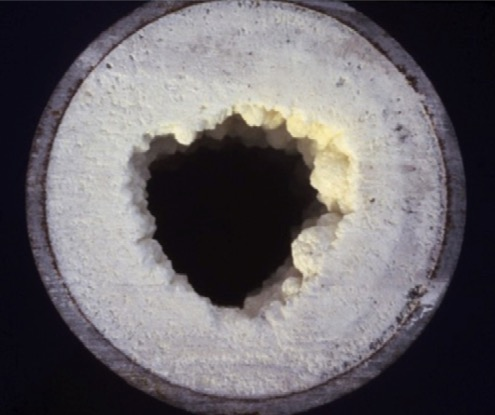
\includegraphics[scale=0.4]{calcim.jpeg}
    \caption{Calcite scaling in a well after three weeks \cite{brown2013mineral}}
    \label{fig:calcl}
\end{figure}
\section{Prevention: CaCO$_3$ scaling}
\newline \newline

In order to prevent calcium carbonate scaling, prevention menthods can be designed and tailored depending upon the site  and the conditions at the site. There are mainly three ways to avoid calicum carbonate scaling: 
\begin{itemize}
    \item acting on CO$_2$ partial pressure 
    \item acting on the pH of the solution 
    \item using chemical additives 
\end{itemize}

However, it is important to emphasize that prevention is not been considered into an extent for this research project since it was out of scope for this report. 
% Add a bit more about sulphate and silicate scaling 
\section{Silica Scaling and prevention}
\newline \newline

Silica scaling is often found in high-temperature resources mainly in the wells and the re-injection lines. There are two types of common silica scaling: amorphous silica and quartz and are often found especially in countries like Italy and El Salvador with high geothermal gradient. As for carbonate scaling, calcite, aragonite and dolomite were considered to be in equilibrium with the geothermal fluid, however for silica scaling quarts is considered to be in equilibrium with the fluid. As the amount of quartz increases with temperature the solubility of quarts is independent of pH. \cite{corsi1986scaling}

As mentioned, silica scaling can be reduced or even eliminated by changing the pH of the solution by adding either HCl or NaOH to the brine fluid. However,this can lead to a huge cost investment and may not be a prefered solution in this case. 
\newline \newline
Due to the complexity of the kinetics of silica polymerization, they are not considered in the report. 
\section{Other types of scaling}
Apart from carbonate and silica, sometimes heavy metal sulphade scaling is observed in production wells which arises due to the sudden pressure decrease of the brine solution which in turn also changes the pH. Again, these are not discussed in this report for the sake of simplicity.  